\documentclass{article}

\usepackage[spanish]{babel}
\usepackage[numbers,sort&compress]{natbib}
\usepackage{graphicx}
\usepackage{url}
\usepackage{amsmath}
\usepackage{hyperref}
\usepackage[top=30mm, bottom=40mm, left=15mm, right=15mm]{geometry}
\setlength{\parskip}{2mm}
\setlength{\parindent}{0pt}

\author{Fulano Tal}
\title{Reporte de prueba}
\date{\today}

\begin{document}

\maketitle

\begin{abstract}

Hola.

\end{abstract}

\section{Introducción}

Hola, dijo \citet{lol}, otra vez. 

La definición de mi fórmula es él de la ecuación \eqref{fx}
\begin{equation}
f(x) = \sum_{i = 1}^n \log_2(x)
\label{fx}
\end{equation}
pero no lo voy a usar para nada. Lo que sí quiero mencionar es el cuadro \ref{esto} y las figuras \ref{flor} y \ref{mono}.

\begin{table}
\caption{Aquí describo el contenido de mi cuadro.}
\label{esto}
\vspace*{3mm}
\centering
\begin{tabular}{lc|r|}
$x$ & hola & 0.02 \\
\hline
$y$ & mundo & 100.12
\end{tabular}
\end{table}

\section{Conclusiones}

Jesús \citep{lol} ayuna cuarenta días y es tentado por el diablo --- Jesús anuncia en Nazaret Su origen divino y es rechazado --- Echa fuera un demonio en Capernaúm, sana a la suegra de Pedro, y predica y sana en toda Galilea.

Jesús ayuna cuarenta días y es tentado por el diablo --- Jesús anuncia en Nazaret Su origen divino y es rechazado --- Echa fuera un demonio en Capernaúm, sana a la suegra de Pedro, y predica y sana en toda Galilea.
Jesús ayuna cuarenta días y es tentado por el diablo --- Jesús anuncia en Nazaret Su origen divino y es rechazado --- Echa fuera un demonio en Capernaúm, sana a la suegra de Pedro, y predica y sana en toda Galilea.
Jesús ayuna cuarenta días y es tentado por el diablo --- Jesús anuncia en Nazaret Su origen divino y es rechazado --- Echa fuera un demonio en Capernaúm, sana a la suegra de Pedro, y predica y sana en toda Galilea.
Jesús ayuna cuarenta días y es tentado por el diablo --- Jesús anuncia en Nazaret Su origen divino y es rechazado --- Echa fuera un demonio en Capernaúm, sana a la suegra de Pedro, y predica y sana en toda Galilea.


Jesús ayuna cuarenta días y es tentado por el diablo --- Jesús anuncia en Nazaret Su origen divino y es rechazado --- Echa fuera un demonio en Capernaúm, sana a la suegra de Pedro, y predica y sana en toda Galilea.
Jesús ayuna cuarenta días y es tentado por el diablo --- Jesús anuncia en Nazaret Su origen divino y es rechazado --- Echa fuera un demonio en Capernaúm, sana a la suegra de Pedro, y predica y sana en toda Galilea.
Jesús ayuna cuarenta días y es tentado por el diablo --- Jesús anuncia en Nazaret Su origen divino y es rechazado --- Echa fuera un demonio en Capernaúm, sana a la suegra de Pedro, y predica y sana en toda Galilea.
Jesús ayuna cuarenta días y es tentado por el diablo --- Jesús anuncia en Nazaret Su origen divino y es rechazado --- Echa fuera un demonio en Capernaúm, sana a la suegra de Pedro, y predica y sana en toda Galilea.

Jesús ayuna cuarenta días y es tentado por el diablo --- Jesús anuncia en Nazaret Su origen divino y es rechazado --- Echa fuera un demonio en Capernaúm, sana a la suegra de Pedro, y predica y sana en toda Galilea.

Jesús ayuna cuarenta días y es tentado por el diablo --- Jesús anuncia en Nazaret Su origen divino y es rechazado --- Echa fuera un demonio en Capernaúm, sana a la suegra de Pedro, y predica y sana en toda Galilea.

Jesús ayuna cuarenta días y es tentado por el diablo --- Jesús anuncia en Nazaret Su origen divino y es rechazado --- Echa fuera un demonio en Capernaúm, sana a la suegra de Pedro, y predica y sana en toda Galilea.
Con madre los flores.




\begin{figure}
\centering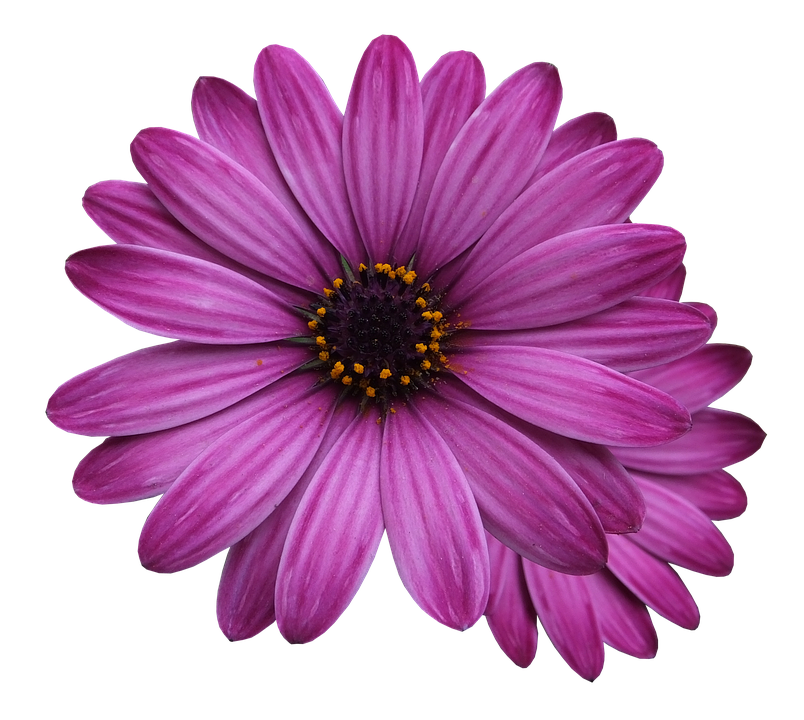
\includegraphics[width=46mm]{flor.png}
\caption{Un flor.}
\label{flor}
\end{figure}


\begin{figure}
\centering
\includegraphics[width=46mm]{mono.jpg}
\caption{Un mono tomado de \url{https://es.wikipedia.org/wiki/Archivo:Mono_pensador.jpg}.}
\label{mono}
\end{figure}



\bibliographystyle{plainnat}
\bibliography{biblio}

\end{document}